\section{Evaluation}
So far, we have presented a sound procedure and automated component-based framework for extracting non-functional properties of generated code. In this section, we evaluate the implementation of our approach by explaining the design of our empirical study; the research questions we set out to answer, the different methods we used to answer these questions. The experimental material is
available for replication purposes at [ref].

\subsection{Research questions}
Our experiments aim at answering the following research questions:

\textbf{RQ1: Mono-objective SBSE Validation.} 
\textit{How does the proposed diversity-based exploration of optimization sequences perform compared to other mono-objective algorithms in term of memory consumption, CPU, execution time, etc.?} 
In this experiment, we generate a set of random Csmith programs \textit{"the training set"} and apply different mono-objective algorithms to assess the different non-functional properties of produced binaries. We compare as well manually generated sequences to standard GCC optimization levels. Our quality metric in this experiment is the percentage of overall performance improvement across all programs under test. The goal of this initial experiment is to: (1) evaluate the effectiveness of our component-based infrastructure to extract non-functional properties such as memory and CPU consumptions; (2) evaluate the performance of our proposed diversity-based exploration of optimization sequences (NS) to GA and RS; and finally (3) find the optimal solution relative to the input training set. 

\textbf{RQ2: Sensitivity.} 
\textit{How sensitive are benchmark programs to compiler optimization options?}
Another interesting experiment is to test the sensitivity of training set programs to best optimal sequence previously discovered in RQ1. To do so, we apply best discovered optimizations to new unseen Csmith and CBench programs and compared the performance results. The idea of this experiment is to test if only Csmith programs are sensitive to compiler optimizations. If so, this will be useful for compiler users and researchers to use GENECO in order to build general optimization sequences from their representative training set programs.


\textbf{RQ3: Impact of optimizations on resource consumption.} 
\textit{How compiler optimizations impact on the non-functional properties of generated programs?}
To answer this question, we use GENECO to generate best sequences per-Benchmark in term of speedup, and compare the memory footprint and CPU consumption of best optimized code. The goal of this experiment is to provide an understanding of the resource consumption of generated code by GCC. 

\textbf{RQ4: Trade-offs between non-functional properties.} 
\textit{How can multi-objective approaches be useful to find trade-offs between non-functional properties?}
A multi-objective approach provides a trade-off between the two objectives
where the developers can select their desired solution from the Pareto-optimal front. The goal of this experiment is to put more emphasis on resource consumption and use multi-objective algorithms to find trade-offs between non-functional properties of generated code like $<$ExecutionTime--MemoryUsage$>$, etc.


All these experiments are conducted using GENECO and they enable us to validate our global approach for non-functional testing of code generators using system containers. 

\subsection{Setup and Methodology}
\subsubsection{Programs used in the empirical study}
To explore the impact of compiler optimizations a set of input programs are needed. 
To do so, we used a random C program generator called Csmith \cite{yang2011finding}.
Csmith is a tool that can generate random C programs that statically and dynamically conform to the C99 standard. It has been widely used to perform functional testing of compilers \cite{le2014compiler} \cite{nagai2013scaling}. Csmith can generate C programs that utilize a much wider range of C features including complex control flow and data structures such as pointers, arrays, and structs. Csmith programs come with their test suites that explore the structure of generated programs. 
Authors argue that Csmith is an effective bug-finding tool because it generates tests that explore atypical combinations of C language features. They argue as well that larger programs are more effective for functional testing. Thus, we run Csmith for 24 hours and gathered the largest generated programs. We depicted 20 C programs with average source lines 12K.

As well, we run experiments on commonly used benchmarks in iterative compilation named Collective Benchmark (cBench)~\cite{fursin2009collective}. It is a collection of open-source sequential programs in C targeting specific areas of the embedded market. It comes with multiple datasets assembled by the community to enable realistic benchmarking and research on program and architecture optimization. cBench contains more than 20 C programs. 
\iffalse
\begin{table}[h]
	\begin{center}
		\begin{tabular}{|c|c|p{3.9cm}|}
			\hline
			\textbf{Program} & \textbf{Source lines} & \textbf{Description}\\
			\hline
			automative\_susan\_s & 1376 & Image recognition package\\
			\hline
			bzip2e & 5125 & Compress any file
			source code \\
			\hline
			bzip2d & 5125 & Decompress zipped files \\
			\hline
			office\_rsynth & 4111 & Text to speech program produced by integrating various pieces of code\\
			\hline
			consumer\_tiffmedian& 15870 & Apply the median cut algorithm to data in a TIFF file
			\\
			
			\hline
			consumer\_tiffdither& 15399 & Convert a greyscale image to bilevel using dithering
			\\
			\hline
			
		\end{tabular}
		
	\end{center}
	\caption {Description of selected benchmark programs}
\end{table}
\fi
\subsubsection{Parameter Tuning and Setting}
%Our experiments use the classical NS algorithm, where we evolve a set of optimization sequences through generations.
NS is implemented as described in Section 3.
The first step in the process of selection is to evaluate each individual and compute its novelty score. Novelty is calculated for each organism by taking the mean of its 15 lowest dissimilar optimization sequences (considering all sequences in the current population and in the archive). 
Then, to create next populations, an elite of the 10 most novel organisms is copied unchanged, after which the rest of the new population is created by tournament selection according to novelty. Standard genetic programming crossover and mutation operators are applied to these novel sequences in order to produce offspring individuals and fulfill the next population.
In the meanwhile, individuals that get a score higher than the threshold T they are automatically added to the archive as well. 
In fact, this threshold is dynamic. Every 150 evaluations, we check how many individuals have been copied into the archive. If this number is below 3, the threshold is increased by multiplying it by 0.95, whereas if solutions added to archive are above 3, the threshold is decreased by multiplying it by 1.05. 
Moreover, as the size of the archive grows, the nearest-neighbor calculations that determine the novelty scores for individuals become more computationally demanding. So to avoid having low accuracy of novelty, we choose to bound the size of the archive. Hence, it follows a first-in first-out data structure which means that when a new solution gets added, the oldest solution in the novelty archive will be discarded. Thus, we ensure individuals diversity by removing old sequences that may no longer be reachable from the current population.

The parameters of the algorithm were tuned individually in preliminary experiments. For each parameter, a set of values was tested. The parameter values chosen are the mostly used in the literature~\cite{lehman2008exploiting}. The value that yielded the highest performance scores was chosen. The resulting parameter values are listed in Table 4.
\begin{table}
	\caption{Parameters of NS algorithm}
	\begin{tabular}{ l l || l l }
		Parameter & Value & Parameter & Value \\	\hline
		Novelty nearest-k  & 15 &  Tournament size & 2\\ 
		Add archive prob. & 30 &  Mutation prob. & 0.1\\  
		Max archive size & 500 &  Crossover & 0.5  \\  
		Population size & 100 &  Nb generations &  100 \\  
		Individual length & 76 & Elitism & 10  \\ 
		Scaling archive prob. & 0.05 & Solutions added to archive & 3  \\ 
	\end{tabular}
\end{table}

\subsubsection{Evaluation Metrics Used}
When comparing two mono-objective algorithms, it is usual to
compare their best solutions found so far during the optimization
process. However, this is not applicable when comparing two multi-objective
evolutionary algorithms since each of them gives as output
a set of non-dominated (Pareto equivalent) solutions. For this reason,
we use performance indicator to compare multi-objective algorithms.
For mono-objective algorithms we used to evaluate solutions using the following metrics:

-\textit{Memory Consumption Reduction (MR)}: corresponds to the percentage ratio of memory usage reduction of running container over the baseline. The baseline in our experiments is the amount of memory usage at O0 level with no optimizations. Larger values for this metric mean better performance. Memory usage is measured in bytes.

-\textit{CPU Consumption Reduction (CR)}: corresponds to the percentage ratio of CPU usage reduction over the baseline. Larger values for this metric mean better performance. The CPU consumption is measured as the CPU time in seconds.

-\textit{Speedup (S)}: corresponds to the percentage improvement in speed of execution of an optimized code compared to execution time of baseline version. Programs execution time is measured in seconds.

For multi-objective algorithms we used to evaluate solutions using the following metric:

-\textit{Hypervolume (HV)}: corresponds to the proportion of the objective space that is dominated by the Pareto front approximation returned by the algorithm and delimited by a reference point. The HV reference point is the point obtained by taking the maximum value observed. Thus, the HV metric can be computed as the area between the Pareto frontier and the HV reference point. Larger values for this metric mean better performance. The most interesting features of this indicator are its Pareto dominance compliance and its ability to capture both convergence and diversity\cite{deb2001multi}. 

\subsubsection{Setting up infrastructure}
To answer previous research questions, we configure GENECO to run different experiments. Figure 2 shows a big picture of the testing and monitoring infrastructure considered in these experiments. 
First a meta-heuristic (mono or multi-objective) is applied to generate specific optimization sequences for the GCC compiler (step 1). During our experiments, we used GCC 4.8.4 as it is introduced in the motivation section but it is possible to choose another compiler versions using GENECO since the process of extracting compiler optimizations is done automatically. As we are applying an evolutionary process, the new generated sequence have to be compiled and executed to gather performance metrics. We apply then the new generated optimization sequence to the input program under test (PUT) and deploy the output binary within a new instance of docker image (step 2). While executing the optimized code inside the container, performance data are sent the monitoring container (step 4) and recorded in a new times series database using our InfluxDB back-end container (step 5). Then, GENECO accesses remotely to stored data in InfluxDB using a REST API and assigns a new performance value to the current solution(step 6). The choice of performance metric depends on experiment objectives (Memory or CPU usage, execution or compilation time, etc.).
\begin{figure}[h]
	\centering
	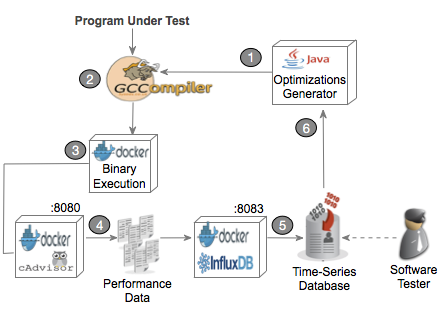
\includegraphics[width=0.9\linewidth]{Ressources/infraup.png}
	\caption{Overview of the Docker-based testing architecture}
\end{figure}
To answer the first research question RQ1, we implement three mono-objective algorithms GA and RS as well our NS adaptation for optimization sequences generation. As it is shown on the left side of figure 3, we used GENECO to search for best optimization sequence from a set of input programs. For this reason, we generated 10 random programs using Csmith \textit{"training set"} and apply the generated sequences to these programs. Thus, the code quality objective function in this
experiments is equal to the average individual performance fitness values for all programs under test. The non-functional property could be CR, MR or S. It depends on the user design choice.

To test the generality of the best optimizations discovered, we apply in RQ2 these sequences to new unseen programs as it is shown on the right part of figure 3. We choose to apply optimizations to new 10 Csmith and 10 Cbench programs. Through this experiment, we would like to test the sensitivity of input programs and general applicability of optimization sequences.

To answer RQ3, we study the impact of these optimizations on memory and CPU consumption using our Docker-based infrastructure. Following again a mono-objective approach, we try in this experiment to maximize the speedup \textit{S} and study in the mean time the impact of \textit{S} on resource consumptions namely memory and CPU usage. In this experiment, we choose 5 Cbench programs to investigate resource consumptions per-benchmark.

Finally in RQ4, we try to use GENECO to find trade-offs between non-functional properties. In this experiment, we choose to focus on the trade-off $<$ExecutionTime--MemoryUsage$>$. We report the comparison results of three multi-objective algorithm adaptations NSGA-II, RS and NS. 
Sequences evaluation is done across 5 Cbench programs as it is conducted in RQ1.
We evaluate the quality of the obtained Pareto optimal optimization levels, both qualitatively by visual inspection of the Pareto frontiers, and quantitatively by using the HV metric.
\begin{figure}[h]
	\centering
	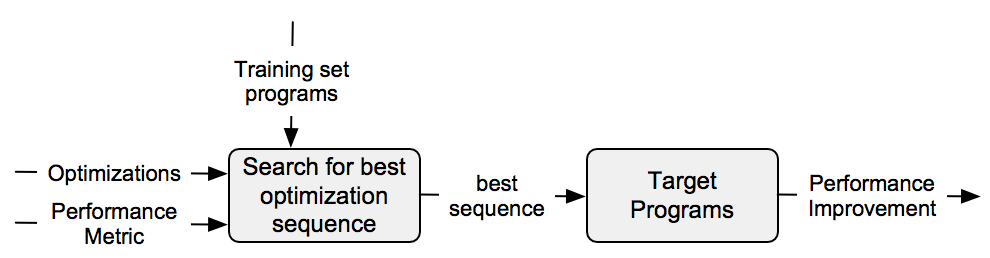
\includegraphics[width=1.\linewidth]{Ressources/sensitivity.png}
	\caption{fig}
\end{figure}

To obtain comparable and reproducible results, we use the same hardware across all experiments: an AMD A10-7700K APU Radeon(TM) R7 Graphics processor with 4 CPU cores (2.0 GHz), running Linux with a 64 bit kernel and 16 GB of system memory.


\subsection{Experimental Results}
In the following paragraphs, we report the results of our experiments.
\subsubsection{RQ1. Mono-objective SBSE Validation}
The goal of thus experiement is to 
\begin{table}[h]
	\centering
	\caption{My caption}
	\label{my-label}
	\begin{tabular}{|l|l|l|l|l|l|l|c|}
		\hline
		& O1                    & O2                    & O3                    & Ofast                 & RS                    & GA                    & NS \\ \hline
		S  & \multicolumn{1}{c|}{} & \multicolumn{1}{c|}{} & \multicolumn{1}{c|}{} & \multicolumn{1}{c|}{} & \multicolumn{1}{c|}{} & \multicolumn{1}{c|}{} &    \\ \hline
		MR &                       &                       &                       &                       &                       &                       &    \\ \hline
		CR &                       &                       &                       &                       &                       &                       &    \\ \hline
	\end{tabular}
\end{table}
\subsubsection{RQ2. Sensitivity}
\subsubsection{RQ3. Impact of optimizations on resource consumption}
\begin{figure}[h]
	\centering
	\includegraphics[width=1.\linewidth]{Ressources/infra_novelty_stat2.png}
	\caption{Evaluating the speedup after applying standard optimization options compared to best generated optimization using NS}
\end{figure}
\subsubsection{RQ4. Trade-offs between non-functional properties}
In this section, we compare our NS adaptation for optimizations generation to the current, state-of-the-art multi-objective approaches namely NSGA-II and RS. Two tradeoffs are investigated in this section; $<$execution time--memory usage$>$ and $<$execution time--CPU usage$>$.

First, we conduct a quantitative study by comparing the HV metric for both tradeoffs than we conduct a quantitative study through pareto front distribution charts.
\subsection{Discussions}










\begin{figure}[!t]
	\centering
	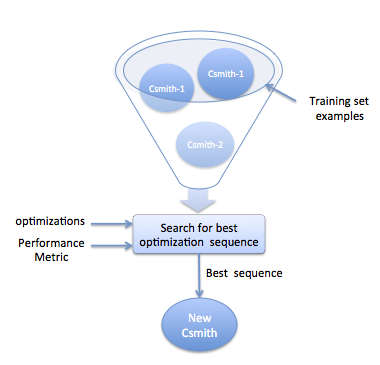
\includegraphics[width=1\hsize]{Ressources/approach by example.png}
	\caption{fig}
\end{figure}

\begin{figure}[!t]
	\centering
	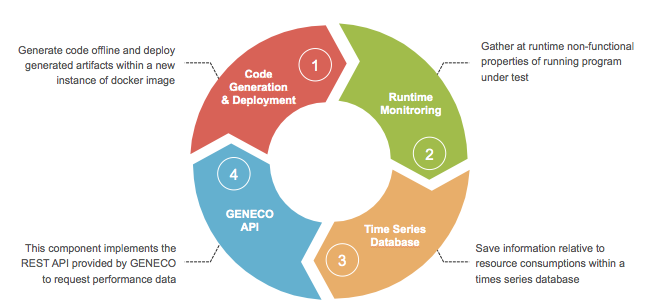
\includegraphics[width=1\hsize]{Ressources/geneco approach.png}
	\caption{fig}
\end{figure}

\begin{figure}[!t]
	\centering
	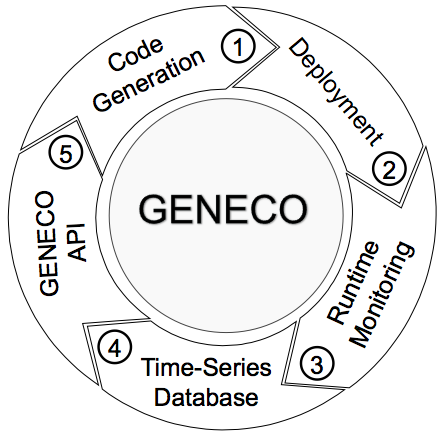
\includegraphics[width=1\hsize]{Ressources/genecoApproach22.png}
	\caption{fig}
\end{figure}
\iffalse
\begin{table}[]
	\centering
	\caption{My caption}
	\label{my-label}
	\begin{tabular}{@{}|l|c|c|c|c|c|c|c|c|c|c|c|c|c|c|c|c|c|c|c|c|@{}}
		\toprule
		\multirow{2}{*}{} & \multicolumn{2}{c|}{CB1} & \multicolumn{2}{c|}{CB2} & \multicolumn{2}{c|}{CB3} & \multicolumn{2}{c|}{CB4} & \multicolumn{2}{c|}{CB5} & \multicolumn{2}{c|}{CS1} & \multicolumn{2}{c|}{CS2} & \multicolumn{2}{c|}{CS3} & \multicolumn{2}{c|}{CS4} & \multicolumn{2}{c|}{CS5} \\ \cmidrule(l){2-21} 
		& Ox & Best & Ox & Best & Ox & Best & Ox & Best & Ox & Best & Ox & Best & Ox & Best & Ox & Best & Ox & Best & Ox & Best \\ \midrule
		Execution Speedup & \begin{tabular}[c]{@{}c@{}}4\%\\ (O3)\end{tabular} &  &  &  &  &  &  &  &  &  &  &  &  &  &  &  &  &  &  &  \\ \midrule
		Memory & \begin{tabular}[c]{@{}c@{}}4\%\\ (O3)\end{tabular} &  &  &  &  &  &  &  &  &  &  &  &  &  &  &  &  &  &  &  \\ \midrule
		CPU & \begin{tabular}[c]{@{}c@{}}4\%\\ (O3)\end{tabular} &  &  &  &  &  &  &  &  &  &  &  &  &  &  &  &  &  &  &  \\ \midrule
		Compilation Speedup &  &  &  &  &  &  &  &  &  &  &  &  &  &  &  &  &  &  &  &  \\ \midrule
		Code Size &  &  &  &  &  &  &  &  &  &  &  &  &  &  &  &  &  &  &  &  \\ \bottomrule
	\end{tabular}
\end{table}
\fi


\begin{figure}[h]
	\centering
	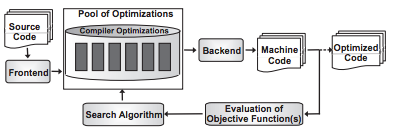
\includegraphics[width=1\hsize]{Ressources/compilation.png}
	\caption{fig}
\end{figure}
\begin{figure}[h]
	\centering
	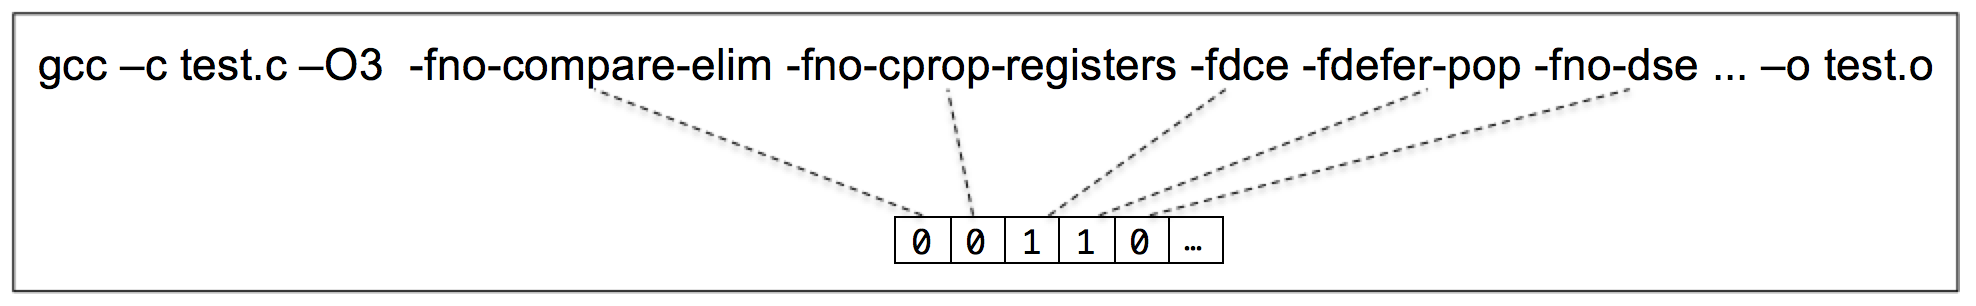
\includegraphics[width=1\hsize]{Ressources/individual.png}
	\caption{fig}
\end{figure}

